\documentclass[crop,tikz]{standalone}
\usepackage{tikz}
\usepackage{xcolor}

\definecolor{ElderGold}{RGB}{255, 215, 0}
\definecolor{ElderBlue}{RGB}{65, 105, 225}
\definecolor{ElderRed}{RGB}{205, 92, 92}

\begin{document}
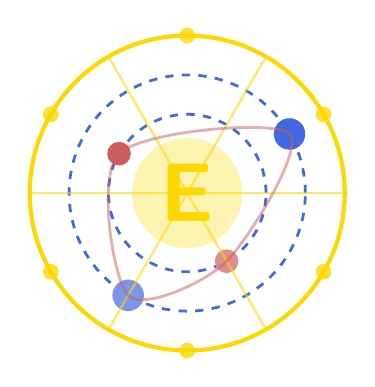
\begin{tikzpicture}

% Outer circle
\draw[line width=1.5pt, ElderGold] (0,0) circle (2cm);

% Inner orbital circles
\draw[line width=1pt, ElderBlue, dashed] (0,0) circle (1.5cm);
\draw[line width=1pt, ElderBlue, dashed] (0,0) circle (1cm);

% "E" symbol in the center
\begin{scope}
\clip (0,0) circle (0.7cm);
\fill[ElderGold!30] (0,0) circle (0.7cm);
\end{scope}
\node[font=\sffamily\bfseries, scale=3, text=ElderGold] at (0,0) {E};

% Orbital bodies
\fill[ElderBlue] (30:1.5cm) circle (0.2cm);
\fill[ElderRed] (150:1cm) circle (0.15cm);
\fill[ElderBlue!70] (240:1.5cm) circle (0.2cm);
\fill[ElderRed!70] (300:1cm) circle (0.15cm);

% Radial lines
\foreach \angle in {0, 60, 120, 180, 240, 300} {
    \draw[line width=0.8pt, ElderGold, opacity=0.6] (0,0) -- (\angle:2cm);
}

% Phase markers
\foreach \angle in {30, 90, 150, 210, 270, 330} {
    \fill[ElderGold, opacity=0.8] (\angle:2cm) circle (0.1cm);
}

% Connecting paths
\draw[ElderRed, opacity=0.5, line width=1pt] plot [smooth cycle] coordinates {(30:1.5cm) (150:1cm) (240:1.5cm) (300:1cm)};

\end{tikzpicture}
\end{document}